%%%%%%%%%%%%%%%%%%%%
% INTRODUCTION
%%%%%%%%%%%%%%%%%%%%
\section{Introduction}
\label{sec:introduction}
%
This paper explores the challenges in providing fault isolation
through memory protection on resource constrained embedded systems
such as sensor nodes.
%
%Sensor networks have promise for many industrial, commercial, and
%medical applications.
%
%For example, CodeBlue~\cite{welsh04codeblue} is a prototype medical
%sensor network platform for expediting triage during disaster
%response.
%
%A network of 4000 sensors deployed by Intel in a
%semiconductor fabrication plant performs predictive maintenance of
%machinery in service~\cite{intel05fabapp}.
%
%The Zigbee consortium~\cite{zigbee} seeks to equip lighting and
%HVAC controllers with wireless radios, enabling intelligent building
%automation and security services.
%
%These 
Current and upcoming sensor network deployments require high
availability infrastructure with the ability to support multiple users.
%
%
Unexpected system failures could cause problems ranging from financial
impacts to loss of life.
%
Current software technology is grossly inadequate to run such long
term deployments.
%
Bugs in any part of the software can easily bring down an entire network.
%
In particular, memory corruption due to buggy applications can crash or
freeze sensor nodes or corrupt sensed data.
%
We argue that memory protection is a vital enabling technology for
creating reliable and long-lasting sensor network software systems.
%

Sensor software is quite complex, supporting 
%
many sensor types, multiple distributed
middleware services, dynamic code updates, and concurrent applications.
%
Programmers must deal with severe resource constraints and concurrency issues
%
on hardware with very limited debugging support.
%
Therefore, programming errors are quite common and can impact the network.


Mote-class sensor nodes~\cite{jasonhillthesis} have a very simple architecture.
%
All primary memory is accessible to all programs running
on a node via a single address space.
%
Common mote-class architectures do not have features such as memory
management units (MMUs) and privileged-mode execution used in
desktop/server class systems to isolate program data and code.
%
Embedded microcontroller designers face extreme pressure to minimize chip cost and area.
%
Sometimes even 32-bit ARM processor cores omit an MMU to minimize system cost and power~\cite{arm7tdmi}.
%
We expect MMU designs will continue to be absent from low-cost low-power
microcontrollers.
%
Therefore, there is a need for new advancements in software and architecture
technology to make robust sensor node applications.
%
%==================================================================
%\subsection{Memory Protection in Embedded Sensor Systems}
%
%Software-based approaches for memory protection have emerged to
%compensate for the architectural limitations of embedded
%microcontrollers.
%
%Domain specific interpreters such as Mat\'e~\cite{asvm05nsdi} provide
%a safe environment to execute high-level application scripts.
%
%Type-safe languages such as Virgil~\cite{titzer06virgil} provide
%fine-grained protection of individual memory objects.
%
%However, these approaches have their limitations.
%
%For example, Mat\'e instructions are implemented in non type-safe
%language and could be buggy.
%
%Type-safe languages require unsafe extensions to interface to the
%low-level hardware, though these extensions could be used sparingly.
%
%An ideal system for memory protection might combine two or
%more software-based approaches.
%


In this paper, we present \emph{Harbor}, a system for providing
%software-based 
coarse-grained memory protection in resource-%
constrained embedded sensor nodes.
%
%Harbor can be used as a building block with other approaches to create
%more effective protection mechanisms.
%
%For instance, Harbor can be used to implement memory safe Mat\'e
%instructions.
%
Harbor partitions a sensor node's memory into
multiple \textit{domains}.
%
Memory belonging to one domain is protected from corruption by code running
in other domains.
%
We achieve memory protection by enforcing restrictions on memory accesses.
%
In this paper, we have designed two systems that introduce these restrictions.
%
The first system re-writes machine instructions of a compiled binary.
%
This software only technique, first proposed by Wahbe et
al.~\cite{wahbe93sfi}, is known as software-based fault isolation,
SFI, or ``sandboxing''.
%
The second system modifies the processor architecture to enforce memory
access restrictions and is applicable to system-on-chip embedded
systems using processor cores.
%

%==================================================================
\subsection{Contributions of the Paper}
%
We improve the reliability of embedded sensor software by isolating
the domains from one another.
%
This paper investigates the challenges in implementing fault isolation
on resource-constrained embedded sensor nodes.
%
Scarce memory resources require Harbor to have a very small memory
footprint.
%
Limited computational capabilities also encouraged us to limit Harbor's
CPU overhead.
%
The contribution of our work has been to design techniques that make
sandboxing feasible on embedded sensor nodes despite these
constraints.
%
In particular, these techniques are:
%
\begin{itemize}
%
\item{A \emph{Memory map} data structure that efficiently maintains
fine-grained ownership and layout information for the entire address
space.
%
Motes' limited address space precludes static address space
partitioning: there is not enough memory available to assign each
domain a single contiguous range of addresses.
%
The memory map can be tuned to match available resources and protection
requirements.
%
}
%
\item{A \textit{Safe stack} in protected memory preserves control flow
integrity~\cite{xfi06osdi} within a domain by storing function return addresses.
%
The conventional run-time stack, which stores local data, function
parameters, and so forth and is shared by all the domains, is
protected from corruption via \emph{stack bounds}.
%
The alternative of maintaining a separate stack per
domain is not desirable due to address space limitations.
%
}
%
\item{\textit{Cross domain calls} implement low-overhead
context switches between domains.
%
The overhead of copying call arguments is eliminated as the domains
share a common run-time stack.
%
Cross domain calls and returns track the system's currently active domain.
%
}
%
\item{\textit{Run-time checks} ensure that control flow in and out
of a domain occur as expected even on computed transfers, and
similarly that memory is accessed only as expected.
%
}
%
\end{itemize}

%Figure~\ref{fig:sys_comp} presents the components of the Harbor memory
%protection system and the interactions between them.
%
These techniques are easily incorporated into existing systems.
%
We have designed and evaluated two systems that use the Harbor fault isolation
techniques.
%
Our experiments show that memory protection through fault isolation is
feasible on resource constrained sensor nodes.

% \begin{figure}[htbp]
%     \centering
%     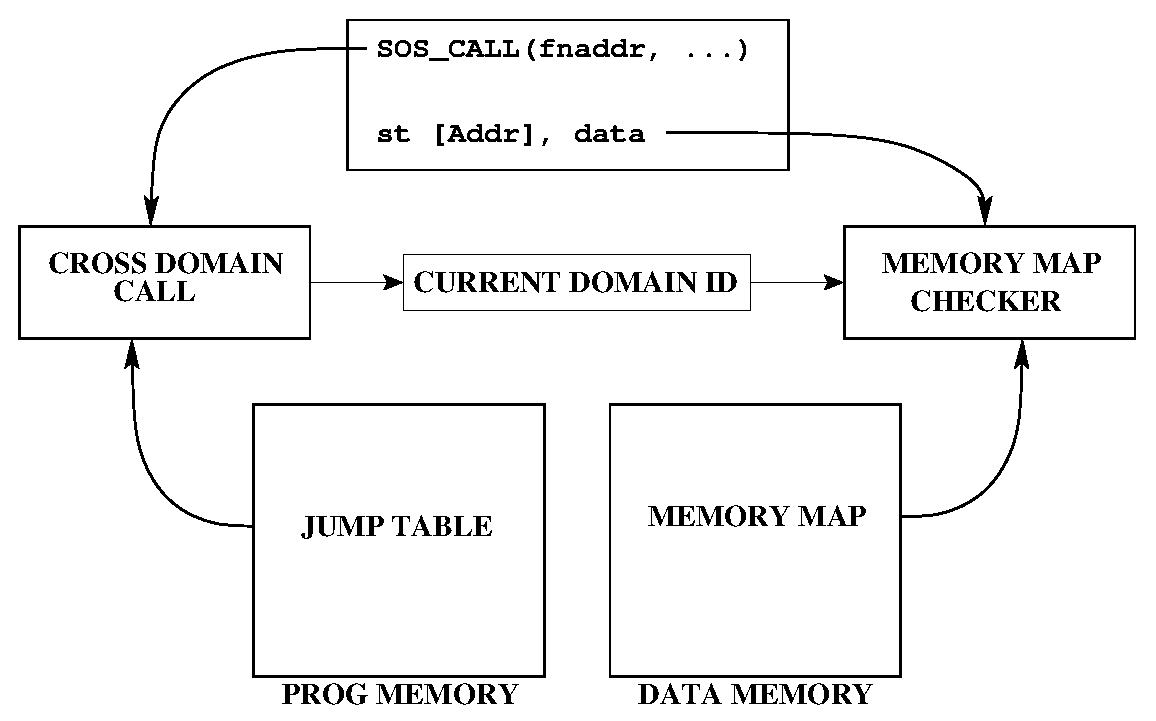
\includegraphics[height = 2.5in, keepaspectratio=true]{figures/syscomp.eps} 
%     \caption{Components of Harbor Memory Protection}
%     \label{fig:sys_comp}
%  \end{figure}

%-------------------------------------------------------
\subsection{Applications of Harbor Memory Protection}
%
\subsubsection{Memory Protection in SOS Operating System}
%
SOS~\cite{ram05sos} is an operating system for sensor nodes in which a
statically compiled kernel is installed on the node, and application
level functionality is implemented by a set of dynamically loadable
binary modules.
%
We use Harbor memory protection to isolate binary modules running
on SOS.
%
Run-time checks are introduced in a SOS module by a \emph{binary rewriter} and
verified independently by a \emph{verifier} running on every sensor
node.
%
To minimize the module code size, the run-time checks are not inlined.
%
Modules invoke the run-time checks by calling or jumping into the
appropriate routines located in the trusted domain (the SOS kernel).
%
%% Thus, it is not possible to circumvent checks as 
All potentially unsafe operations such as stores to memory are replaced
by calls to corresponding checks.
%
%Calls to the checks are introduced by a \emph{binary rewriter} and verified
%independently by a \emph{verifier} running on every sensor node.
%
Harbor's correctness depends only upon the correctness of the
verifier and the Harbor runtime, and not on the rewriter.
%
%The design of the verifier affects the system's performance
%(Section~\ref{sec:writeverify}).
%
%So far, we have only 
We have designed a simple verifier that requires constant state
information for a binary.
%
%Exploring the design space of verifiers and evaluating their impact on
%performance is a challenge that remains to be addressed.
%----------------------------------------------------------------------------
\subsubsection{Micro Memory Protection Unit}
%
We design a Micro Memory Protection Unit (UMPU) by partitioning the
Harbor Memory Protection system into hardware and software components.
%
UMPU was implemented on the AVR~\cite{avrdatasheet} microcontroller and
its performance was evaluated by executing complex software systems
such as SOS.
%
The careful hardware software co-design of UMPU results in significant
performance improvement over a software-only implementation with minimal
increase to the area and cost of AVR.
%
AVR enhanced with UMPU extensions is instruction set compatible with
regular AVR microcontrollers.
%
This design feature has practical value, as the existing
toolchains for the AVR architecture can be used with UMPU.
%
%
%An additional benefit of UMPU is that it eliminates the binary
%rewriting required by the software-only implementation that can be
%error-prone.
%


During experimentation, Harbor detected memory corruption in a data
collection application module that had been in use for several months.
%
A common programming mistake in SOS is to forget to check the error code
returned by a cross-domain function call.
%
In the Surge data collection module~\cite{woo03surge}, under certain
conditions, the invalid result of a failed function call to the Tree
routing module was being used to determine an offset into a buffer.
%
Subsequently, the data was being written to an incorrect memory
location, which would cause some of the nodes in the network to crash.
%
Harbor was successfully able to prevent the corruption and signal the
invalid access.
%


The cross-domain function call described above fails under the rare
condition when the Surge module is loaded on a node before the Tree
routing module.
%
Such conditions can be easily missed during software testing.
%
However, during deployments, the errors caused due to such failures
can have a severe impact on the network.
%
A system that can guarantee memory protection is indispensable for
building robust embedded software.
%

Harbor protection mechanism can be applied in general to a large class
of resource constrained embedded systems.
%
In this paper, we will focus primarily on the application of Harbor
protection to embedded sensor networks.
%
%----------------------------------------------------------------------------
%
%\subsection{Robust Embedded Software}
%
%============================================================
\subsection{Structure of Paper}
%
This paper is structured as follows.
%
Section~\ref{sec:related} gives an overview of related work,
examining previous work on software reliability in sensor networks,
software based fault isolation techniques and hardware based
approaches to memory protection in embedded and desktop systems.
%
%There is also a background on the SOS operating system. 
%and presents an overview of the Harbor memory
%protection primitives and their role in
%system that is designed to sandbox 
%sandboxing the dynamically loadable SOS modules.

Section~\ref{sec:memmap} explains the memory map data structure, which
contains fine grained ownership and layout information for every block
within the address space of the sensor node. 
%
Section~\ref{sec:cfmgr} discusses the Control Flow Manager, which
ensures the integrity of control flow within a protection domain
despite memory corruption localized to a domain.

Section~\ref{sec:writeverify} describes the design and implementation
of a binary rewriter tool that sandboxes SOS modules.
%
The sandboxed modules interact with the Harbor run-time components.
%
There is a detailed discussion on the design space of the verifiers
for a binary rewriter.

Section~\ref{sec:umpu} describes the components of UMPU.
%
There is an in-depth 
%detailed design 
description of all the functional units
within UMPU and their interaction with the software library.

We present detailed performance and resource consumption analysis of
Harbor and UMPU in Section~\ref{sec:eval}.
%
We conclude with a summary of our findings and directions for future
work in Section~\ref{sec:conclude}.
